\documentclass[sigconf,nonacm,prologue,table]{acmart}
\usepackage{listings}

%% labels
%% sections:    "sec"
%% definitions: "def"
%% equations:   "eq"
%% figures:     "fig"
%% tables:      "tab"

%% packages
\usepackage{amsmath}
\usepackage{pgfplots}
\usepackage{subcaption}
\usepackage{commath}
\usepackage[utf8]{inputenc}
\usepackage{graphicx}
\usepackage{svg}
\usetikzlibrary{positioning, arrows.meta, shapes, calc}
%% \usepackage{tikz}

\pagenumbering{arabic}

%% hide ACM reference
\settopmatter{printacmref=false}

%% hide copyright
\renewcommand\footnotetextcopyrightpermission[1]{}

%% \pagestyle{plain}
\settopmatter{printfolios=true}

\numberwithin{equation}{section}

\theoremstyle{definition}
\newtheorem{definition}{Definition}

\theoremstyle{remark}
\newtheorem*{remark}{Remark}

\captionsetup[subfigure]{
    labelfont=bf,
    textfont=normalfont,
}
\renewcommand{\thesubfigure}{\Roman{subfigure}}

\definecolor{rowA}{gray}{0.9}
\definecolor{rowB}{gray}{0.8}

\newcommand{\rplus}{\mathbb{R}_{\geq 0}}
\newcommand{\rpos}{\mathbb{R}_{>0}}

\begin{document}
\title{Steamm}
\subtitle{November 2024}
\date{November 2024}

\author{Nojob}
\affiliation{}
\email{nojob@solend.fi}

\author{0xxgen}
\affiliation{}
\email{0xxgen@solend.fi}

\author{Ripleys}
\affiliation{}
\email{ripleys@solend.fi}

\begin{teaserfigure}
\caption*{
    \hspace{\textwidth}
    }
\end{teaserfigure}

\renewcommand{\shortauthors}{Adams et al.}

\begin{abstract}

\textsc{Steamm} is an Automated Market Maker with an embedded money market integration, designed to maximize capital efficiency. It features a composable architecture that allows for the integration of various quotation system, such as a Constant-Product quoter, quoters specialized in stablecoin trading, as well as dynamic fee quoters based on market volatility and trading volume.

\textsc{Steamm's} liquidity re-utilization model deposits idle liquidity into Suilend's lending markets, improving capital efficiency and generating additional yield for liquidity providers.
\end{abstract}

\maketitle

\section{Introduction} \label{sec:introduction}

Traditional AMMs often leave liquidity idle, earning yield only when actively used for trades. This results in a significant opportunity cost for Liquidity Providers (LPs). \textsc{Steamm} addresses this inefficiency by introducing a shared liquidity model, allowing unused funds to generate yield in lending markets while remaining accessible for trades.

The protocol’s modular quotation design enables seamless integration of various swap quotation systems. This flexibility accommodates innovation, allowing new quotation models to be added as the DeFi industry evolves. With these features, we combine adaptability and efficiency, offering LPs enhanced earning opportunities and bespoke solutions for traders.

In it's core, the protocol operates on the following objects:
\begin{itemize}
    \item \emph{Pool<A, B, Quoter, LendingMarket>}: Top-level object and sits at the core of the protocol. The generic types \emph{A} and \emph{B} correspond to the associated coin types of the AMM. The \emph{Quoter} type corresponds to the type of the associated quote module. The \empher{Quoter} also stores state. The pool object holds information related to the pool's liquidity, trading data, protocol and pool fees, LP Supply, bToken balances as well as the inner state of the quotation model.
    
    \item \emph{Bank<LendingMarket, T>}: This object sits between the AMM pools and the lending markets. The Bank aggregates all funds of type \emph{Coin<T>} from all corresponding pools. It also manages the relationship between the types \emph{Coin<T>} and \emph{Coin<BToken<T>>}.
\end{itemize}

Note that the pool holds bTokens and handle swaps through them. By holding bTokens, Pools will accrue interest accumulated from the bank's lending operations, interest which is then distributed to LPs, throughout the LP redemption process.

Not all coin types will have a liquid lending market. In such cases, the bank will not deploy them to the money markets and instead will keep the full amount in custody. For such cases, the corresponding bToken is pegged one to one with the respective underlying.

\begin{figure}[htbp]
  \centering
  \includegraphics[width=0.4\textwidth]{assets/flow.png}
  \caption{Liquidity re-utilization flow}
  \label{fig:workflow}
\end{figure}

\section{Bank}
\label{sec:liquidityreutilization}

Banks operate by pooling liquidity from a given coin type and allocating a portion of that liquidity to lending markets, thereby earning yield. By consolidating liquidity, AMM pools can fulfill their swap commitments by tapping into the global net liquidity available in the respective banks, thereby reducing the liquidity recall frequency from lending markets.

For example, if one pool experiences high demand for \emph{SUI} (i.e, a high volume of swaps extracting \emph{SUI} from the pool) and another experiences high supply of \emph{SUI} (i.e., a high volume of swaps adding \emph{SUI} to the pool), these flows will largely offset each other.

In other words, during periods of low market correlation, offsetting flows occur. However, during periods of high market correlation, there is a greater need to recall liquidity from the lending markets.

\subsection{Yield-bearing LP tokens} \label{yieldbearingtokens}
Liquidity re-utilization not only enhances overall market efficiency but also allows liquidity providers to earn a money-market yield on their funds while market-making. Banks deposit funds into the lending market, earning a yield $r$ , that compounds over time. They then act as pass-through entities, distributing the yield to the respective pools in proportion to the time and principal invested.

The bank facilitates this pass-through process by allocating an intermediate bToken to each participating pool. Whenever a pool adds new funds to a bank, the bank issues bTokens in proportion to the new incoming principal relative to the bank’s current value (taking into account both funds on Suilend and funds held in contingency).

\begin{equation}
\Delta{B_{tokens}} = \frac{\Delta{Principal} *B_{supply} }{Principal + Interest}
\tag{2.1}
\end{equation}

In a nutshell, bTokens enable the interest earned to flow back into the pool, where it is added to the liquidity and distributed further to each LP position.
In practice, the effective yield generated on funds allocated to a bank is lower than the lending market yield, as the bank maintains a utilization rate below 100\% to ensure pools can fulfill trades without having to withdraw funds from the lending market.

\begin{figure}[htbp]
  \centering
  \includegraphics[width=0.45\textwidth]{assets/btokens.png}
  \caption{End-to-end flow from LP tokens, to bTokens to cTokens}
  \label{fig:utilization}
\end{figure}

\subsection{Utilization Target and Buffer} \label{utilizationtargetbuffer}

Banks are configured with a target utilization rate. Liquidity deployed to the lending market is allowed to fluctuate around the target utilization rate and the extent to which these fluctuations can deviate from the target is defined by a utilization buffer. So if the target utilization is set at 50\% with a utilization buffer of 5\%, then utilized liquidity is allowed to fluctuate between 45\% and 55\%.

\begin{figure}[htbp]
  \centering
  \includegraphics[width=0.3\textwidth]{assets/utilization.png}
  \caption{Illustration of utilization range}
  \label{fig:utilization}
\end{figure}

These parameters are set by the global admin when lending is initialized. However, they can be updated dynamically, enabling strategies that manage utilization based on market conditions such as volatility and order flow.

The utilization rate $U$ is defined as ratio between deployed liquidity $d$ and total liquidity $L$ (deployed plus available liquidity $a$):

\begin{equation}
U = \frac{d}{L}
\tag{2.2.1}
\end{equation}

where $L = d + a$

When a given inflow or outflow $\Delta L$ occurs, we recompute the post utilization rate, such that for negative flows we recall funds from the lending market if the following condition is met:

\begin{gather*}
    U < U^* - b \\
    \iff \frac{d}{a + d - \Delta L} < U^* - b \\
    \iff d < (U^* - b)(a + d - \Delta L) \; : \; \Delta L < a + d
\tag{2.2.2}
\end{gather*}

Where $b$ stands for the utilization buffer.

The recall amount $\Delta a$ is then computed as follows:

\begin{gather*}
    \frac{d - \Delta a}{a + d - \Delta L} = U^* \\
    \iff \Delta a = d - U^* (a + d - \Delta L)
\tag{2.2.3}
\end{gather*}

In the same way, when flows are positive we deploy funds to the lending market if the following condition is met:

\begin{gather*}
    U > U^* + b \\
    \iff \frac{d}{a + d + \Delta L} > U^* + b \\
    \iff d > (U^* + b)(a + d + \Delta L)
\tag{2.2.4}
\end{gather*}

Where the deploy amount $\Delta d$ is computed as follows:

\begin{gather*}
    \frac{d + \Delta d}{a + d + \Delta L} = U^* \\
    \iff \Delta d = U^* (a + d + \Delta L) - d
\tag{2.2.5}
\end{gather*}

The ability to parameterize utilization allows the protocol to maximize efficiency without compromising on market-making. When market conditions indicate unidirectional volatility, banks can adjust the utilization rate higher or lower, depending on which side of the trading pair is experiencing sell pressure. Conversely, when volatility is relatively symmetric, the utilization rate can be lowered to account for bidirectional flows.

\section{Swap Model}
\label{sec:swapmodel}

Given the yielding nature of the liquidity, swap quotations are applied to the bToken counterparts of each token. This approach allows pools to consider the accumulated interest of each asset as part of the liquidity itself. In practice, when a user swaps, say, \emph{USDC} for \emph{SUI}, the protocol first converts the input amount of \emph{USDC} into an equivalent amount of \emph{BUSDC}, then quotes the output amount in \emph{BSUI}, which is ultimately converted into the corresponding amount in \emph{SUI}.

Since a swap consists of an inflow and a corresponding outflow, a provisioning action occurs before the swap to ensure the pool has sufficient funds to fulfill the outflow. A follow-up action then rebalances the liquidity from the inflow, maintaining the pool’s equilibrium.

\begin{figure}[htbp]
  \centering
  \includegraphics[width=0.4\textwidth]{assets/swapflow.png}
  \caption{Illustration of a swap flow}
  \label{fig:swap}
\end{figure}

The swap model follows an intent/execute pattern where traders start by formalizing an intent to swap with a given pool. During the intent process the pool formulates a quote. The intent object itself is a wrapper around a quote, which its creation signals to the pool that a swap is about to take place.

The core reason behind breaking the swap into this pattern is to allow the banks provision enough liquidity to fulfill the swap. The flow is as follows:

\begin{itemize}
    \item Intent swap: Pool provides a quotation via \\ \verb|quoter_x::intent_swap()|
    \item Based on the intent object, banks provision liquidity as needed
    \item Swap is executed \verb|quoter_x::execute_swap()|
    \item Optionally rebalance the utilization of the bank receiving the inflow
\end{itemize}

\begin{figure}[htbp]
  \centering
  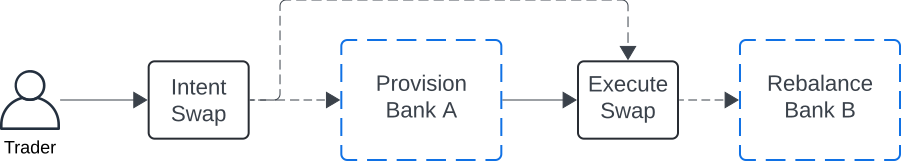
\includegraphics[width=0.4\textwidth]{assets/swap_intent.png}
  \caption{Illustration of a swap intent flow}
  \label{fig:swapintent}
\end{figure}


\section{Liquidity Providers}
\label{sec:lp}
When it regards to the deposit and withdrawal of liquidity by the LPs, the flow is rather straightforward.

When depositing liquidity, the respective banks will optionally deploy extra liquidity to the lending markets to guarantee that utilization bounds are met.

\begin{figure}[htbp]
  \centering
  \includegraphics[width=0.4\textwidth]{assets/depositflow.png}
  \caption{Illustration of a deposit}
  \label{fig:deposit}
\end{figure}

By contrast, when redeeming liquidity, we check if the outflows can be met and if the banks utilization remains within the bounds defined, and if not the banks will recall the required liquidity from the lending markets.

\begin{figure}[htbp]
  \centering
  \includegraphics[width=0.4\textwidth]{assets/withdrawflow.png}
  \caption{Illustration of a withdraw}
  \label{fig:withdraw}
\end{figure}


\section{Quoters}
\label{sec:quoters}

Currently, the protocol has three built-in quotation models: a Constant-Product Quoter, a Stable Quoter, and a volatility-based dynamic-fee Quoter.

To initiate a pool, the base pool module provides a generator function \verb|pool::new()|, for use by the quoter modules to construct the pool. This function allows each quoter to integrate its custom state. The quoter then export in its public interface \verb|quoter_x::new()|.

Similarly, the base module makes the core swap function \verb|pool::swap()| available to the quoters, which are then responsible for re-exporting the swap functionality in its public interface, via \verb|quoter_x::intent_swap()|, \verb|quoter_x::execute_swap()| and \verb|quoter_x::swap()|, the latter wrapping both the intent and the execution in one function call.

This design allows quoters to define a logic before and after the execution of the main logic defined by the pool module.

\subsection{Constant Product Quoter} \label{cpquoter}

The constant-product quoter uses the default constant-product function with an offset. This quoter operates on the principle of preserving the product of the reserves of the two assets in the pool, ensuring that the product remains constant regardless of the trades that occur.

We define the constant-product formula as:

\begin{equation}
x(y+c)=k
\end{equation}

Where:
- $x$ represents the reserve of asset $X$
- $y$ represents the reserve of asset $Y$
- $c$ represents a vertical offset
- $k$ is the invariant product of the reserves

When a trader swaps one asset for another, the constant-product formula is adjusted to reflect the new reserves while maintaining the invariant $k$.

Given a swap, the AMM adjusts the reserves to maintain the invariant. 

Given an input $\Delta x$, the pool will return an output $\Delta y$ such that:

\begin{equation}
y - \Delta y + c = \frac{k}{x + \Delta x}
\end{equation}

Hence:

\begin{equation}
\Delta y = (y + c) - \frac{k}{x + \Delta x}
\end{equation}


Fees are then computed on the output amount $\Delta y$:

\begin{equation}
\text{Fee} = \Delta y \times Fee Rate
\end{equation}

As for the offset, it allows pool creators to initialize a pool with one-sided liquidity. By setting the offset as a non-zero value we are shifting the constant-product curve vertically.

We can therefore define the point at which the curve intercepts the x axis (when $y=0$) as follows:

\begin{gather*}
    x(0+c) = k \\
    \iff xc = k \\
    \iff x = k / c \\
\tag{5.5}
\end{gather*}

\subsection{Stable Quoter} \label{stablequoter}

The Stable Quoter provides a constant price formula for the purpose of trading stable coins. This quoter provides a quotation for trading stables in a fixed range of reserve ratios, defined by the pool. We defined the lower reserve ratio bound $R_l$ and upper reserve ratio bound $R_u$ as follows:

\begin{equation}
R_l = \frac{x_l}{y_l}
\tag{5.2.1}
\end{equation}

Representing the lower bound of the ratio between token $X$ and token $Y$ beyond which the pool no longer offers a quotation.

\begin{equation}
R_u = \frac{x_u}{y_u}
\tag{5.2.2}
\end{equation}

Representing the upper bound of the ratio between token $X$ and token $Y$ beyond which the pool no longer offers a quotation.

\subsection{Dynamic Fee Quoter} \label{dynamicfeequoter}

The Dynamic Fee Quoter provides a quotation mechanism with dynamic fees based on market volatility. When a trader swaps, the quoter computes an exponential-moving average of the volatility based on a reference price and accumulated volatility metric.

We use absolute price deviations as a proxy for volatility. We define the accumulated volatility metric as follows:

\begin{equation}
V_{\lambda} = \max\left(
    \hat{V} + \max(|P_{oracle} - \hat{P}|, |P_{internal} - \hat{P}|),
    \text{MaxVol}
\right)
\tag{5.3.1}
\end{equation}

Where $P_{oracle}$ stands for the oracle price and $P_{internal}$ the internal constant-product price of the pool. The volatility accumulated metric is capped by a parameter $MaxVol$ defined by the pool.

When a swap occurs, at $n+1$, we compute the reference price as well as the reference volatility:


\begin{equation}
\hat{P}_{n+1} = 
\begin{cases} 
P_{oracle} & \text{, } t = 0 \\
\hat{P}_n & \text{, } \Delta t < f \\
P_{oracle} & \text{, } \Delta t \geq f
\end{cases}
\tag{5.3.2}
\end{equation}

\begin{equation}
\hat{V}_{n+1} = 
\begin{cases}
0 & \text{, } t = 0\\
\hat{V}_n & \text{, } \Delta t < f \\
V_{\lambda} \times R & \text{, } \Delta t \geq f \\
0 & \text{, } \Delta t > d
\end{cases}
\tag{5.3.3}
\end{equation}

where
\begin{equation}
\Delta t = \hat{t}_{n} - t
\tag{5.3.4}
\end{equation}

and we update the reference time after the two previous computations such that:

\begin{equation}
\hat{t}_{n+1} = 
\begin{cases}
t & \text{, } t = 0\\
\hat{t}_{n} & \text{, } \Delta t < f \\
t & \text{, } \Delta t \geq f \\
\end{cases}
\tag{5.3.5}
\end{equation}

The quoter then provides a quotation price based on the constant-product formula and adds a dynamic fee charged on the output:

\begin{equation}
\Delta Out \times \frac{V_{\lambda}^2 \times \phi}{100}
\tag{5.3.6}
\end{equation}

Where $\Delta Out$ represents the output amount and $\phi$ is a fee control parameter used for scaling.

\section{Summary} \label{summary}

\textsc{Steamm} is an advanced Automated Market Maker that maximizes liquidity efficiency, through its native money market integration, and adaptability through its modular quotation design. By enabling various swap quotation models, including constant-product, stable, and dynamic-fee AMMs, \textsc{Steamm} supports diverse trading needs, offering robust flexibility and enhanced liquidity management.

A key innovation is \textsc{Steamm's} liquidity re-utilization model. Unlike traditional AMMs where liquidity often sits idle, \textsc{Steamm} channels unused liquidity into lending markets via an abstraction called \emph{Bank}, generating additional yield for liquidity providers. Through the use of \emph{bTokens}, earned yield flows back into liquidity pools, creating extra value for LPs while preserving enough reserve liquidity for active trading.

This modular, yield-enhancing design makes \textsc{Steamm} a powerful protocol for liquidity providers, offering both market-making functionality and improved yield with lower opportunity cost. By balancing reserve availability and yield generation, \textsc{Steamm} ensures an optimized experience for users in the Sui ecosystem, meeting both trading and investment needs efficiently.

\end{document}
\endinput